\label{chap:history}

\newthought{The}~following discusses a handful of selected historical papers that are concerned with either the theory of mesoscale eddies or with the detection/tracking of eddies from \SSH~data.

%\section[\Citeauthoryear{Rhines2006}]{\textbf{Waves and Turbulence on a $\dfdy$-Plane} \citep{Rhines2006}}
\section*{\textbf{Waves and Turbulence on a $\dfdy$-Plane} \citep{Rhines2006}}
\label{sec:hist_rhines}
Rhines investigated the effect of the $\dfdy$-plane on the inverse energy cascade of quasi-2-dimensional atmospheric and oceanic turbulence. At constant $\f$, energy should be cascaded to ever-larger scales until halted by the scale of the domain. This is clearly not the case, as no storm has ever grown to global scale. The presence of a meridional restoring force creates a critical scale beyond which the \textit{turbulent migration of the dominant scale nearly ceases \ldots}. Rossby waves are excited which would in theory eventually give way to alternating zonal jets of width $\frac{U}{\dfdy}$. This scale was later coined the Rhines Scale $\Lb$.

%\section[\Citeauthoryear{Cushman-Roisin1990}]{\textbf{Westward Motion of Mesoscale Eddies} \citep{Cushman-Roisin1990}}\label{sec:hist_cush}
\section*{\textbf{Westward Motion of Mesoscale Eddies} \citep{Cushman-Roisin1990}}\label{sec:hist_cush}
\citet{Bjerknes1944} already noted that the $\dfdy$-effect causes a mass-imbalance in planetary vortices that, if not met by an asymmetry in shape must lead to westward propagation.
\citet{Nof1981} derived that the $\dfdy$-effect results in a net meridional force on the integrated mass of the vortex, which in balance with the Coriolis acceleration shoves cyclones eastward and anti-cyclones westward. They also explained how displaced water outside the eddy's perimeter causes a much stronger westward component, with the result that all eddies propagate westward irrespective or rotational sense.
 The westward drift was also derived in various forms by
\eg~\citet{flierl1984rossby,matsuura1982evolution,VanLeeuwen2007}.

\newthought{The}~paper by \citet{Cushman-Roisin1990} is particularly helpful to understand where the two components of westward drift come from.
By scaling the terms in the one-layer primitive equations by their respective dimensionless numbers, integrating the interface-displacement caused by the eddy over the eddy's domain and applying mass continuity they derive for the location $(X,Y)$ of an eddy's centroid\footnote{$\intms{}\equiv \intm{}$.}:
%%....................................................................
\begin{align}
	\Pi X_{tt} - Y_t
	%&=
	%\frac{\Bu \Ro }{\Rh \Pi} \intms{yv}
	%+
	%\frac{\Ro^2 }{\Rh \Pi} \intms{y\eta v}\\
	%%--------------------------------------------------------------------
	&=
	\Lr T \beta     \intms{yv}
	+
	L\frac{  \beta  }{ f   } \intms{y\eta v} \label{eq:cush1}\\
	%%--------------------------------------------------------------------
	\Pi Y_{tt} - X_t
	%&=
	%-\frac{\Bu \Ro }{\Rh \Pi } \intms{yu}
	%-
	%\frac{\Ro^2 }{\Rh \Pi} \intms{y\eta u}\\
	%%--------------------------------------------------------------------
	&=
	-\Lr T \beta   \intms{yu}
	-
	L\frac{  \beta  }{ f   }  \intms{y\eta u} 	 
\end{align}
%....................................................................
where $\Pi=1/f_0T$.\\
 Hence, independent of balance of forces the eddy's center of mass describes inertial oscillations\footnote{compare to \textit{harmonic oscillator}.} on the $f$-plane, even in the absence of $\dfdy$.
Using geostrophic values for $\vec{u}$ and returning to dimensional variables \eqref{eq:cush1} can be cast into:
%%%....................................................................
%\begin{equation}\begin{split}
	%X_t
	%&=
	%-\frac{\Bu \Ro f T}{\Rh} \intms{\eta}
	%-\frac{\Ro^2 f T}{\Rh} \intms{\eta^2}
	%+\order{\frac{\Bu \Ro f T}{\Rh},\left( fT \right)^{-2}}
%\end{split}\end{equation}
%%%%....................................................................
%%....................................................................
\begin{align}
	\dpr{X}{t}
	&=
	-\frac{\beta g'}{\f_{0}^{2}}
	\frac{\inta{H\eta} + \inta{\eta^{2}/2}}{\inta{\eta}} \nonumber	\\
	&=
	-\beta \left( 	\frac{NH}{f_{0}}  \right)^{2}
	-\frac{\inta{\eta^{2}/2}}{\inta{\eta}}	\label{eq:cushmanDrift}	\\
	&=
	\dpr{\omega_{long}}{k}
	- u_{internal}
	%\left(1 +\frac{1}{H} \frac{ \int  \eta^2 \; \mathrm{d}A	}{2\mathrm{V_e}} \right)
	%+\order{\Lr   T\beta ,\Pi}
	\nonumber
	\end{align}
%%....................................................................

\newthought{The}~first term of the RHS of \eqref{eq:cushmanDrift} represents the \textit{planetary lift}\footnote{see~\cref{box:speed_planlift} from \cref{subsec:speeds}.}, which is identical to the zonal group velocity of long Rossby waves \citep{Cushman-Roisin2010}.
The second term $u_{internal}$ represents the \textit{eddy-internal $\dfdy$-effect} (see~\cref{box:speed_beta}). %\footnote{see also \cref{der:cushDrift}}.
 Note that the first term is always westwards, while the second has sign of $-\eta$, \ie westward for anti-cyclones and eastward for cyclones and that the first is always much larger than the second.

% %%%%%%%%%%%%%%%%%%%%%%%%%%%%%%%%%%%%%%%%%%%%%%%%%%%%%%%%%%%%%%%%%%%%%%%%%%%%%%%%%%%%%%%%%%%%%%%%%%%%%%%%
%\clearpage
%The momentum equations for a reduced gravity model on the $\dfdy$-plane are:
%\begin{align}
%\Dpr{u}{t}
%-
%f v
%&=
%-g' \dpr{\eta}{x}\\
%\Dpr{v}{t}
%+
%f u
%&=
%-g' \dpr{\eta}{y}
%\end{align}

%With mass (volume) conservation  :
%\begin{align}
%\Dpr{h}{t}
%+
%h \left( \dpr{u}{x} + \dpr{v}{y} \right)
%&=
%0 \\
%\dpr{h}{t}
%+
%\vec{u}_{hor} \cdot \nabla h
%+
%h \grad \cdot \vec{u}_{hor}
%&=
%0 \\
%\dpr{h}{t}
%+
%\grad \cdot \left( h \vec{u}_{hor} \right)
%&=
%0
%\end{align}
%where $h = H+\eta$ as the sum of undisturbed layer-thickness and interface displacement.
%Interpreting now the center of volume $\vec{V}(x,y)$ of the anomaly as the lateral position $(X,Y)$ of the vortex \ie
%\begin{align}
%X
%&=
%%\dpr{\inta{x \eta}}{\inta{\eta}}
%\frac{1}{V} \inta{x \eta} \label{eq:X}\\
%Y
%&=
%\frac{1}{V} \inta{y \eta} \label{eq:Y}
%\end{align}

%% ---------
%building first and second time derivatives of \eqref{eq:X} and \eqref{eq:Y} 
%\begin{align}
%V \dpr{X}{t}
%&=
%\inta{x \dpr{\eta}{t}}\\
%&=
%-\inta{x \left( \grad \cdot \left( h \vec{u}_{hor} \right) \right)	} \\
%&=
%\inta{h u} \label{eq:Xt}
%\end{align}
%\TODO{why?}
%% ---------
%respectively
%\begin{align}
%V \dpr{Y}{t}
%&=
%\inta{h v} \label{eq:Yt}
%\end{align}

%and
%% ---------
%\begin{align}
%V \dpr{^{2}X}{t^{2}}
%&=
%\inta{\left( h u  \right)_{t}}\\
%&=
%\inta{
%h u_{t}
%+
%u h_{t}
%}\\
%&=
%\inta{
  %-h g' \eta_{x} + h f v 
%-
%u \left( \grad \cdot \left( h \vec{u} \right) \right)
%}
%\end{align}
%\TODO{terms 1 and 3 of RHS drop. Why?}
%leaving

%\clearpage
%\begin{align}
%V \dpr{^{2}X}{t^{2}}
	%&=
 %\inta{f h v}
%\end{align}

%with \eqref{eq:Yt}:

%\begin{align}
%V \dpr{^{2}X}{t^{2}}
	%&=
 %f \inta{hv}
 %-
 %\inta{\beta \inta{hv}} \\
 %&=
 %f V \dpr{Y}{t}
 %-
 %\inta{\beta V \dpr{Y}{t}} \\
%\dpr{^{2}X}{t^{2}}
  %&=
 %f  \dpr{Y}{t}
 %-
 %\inta{\beta  \dpr{Y}{t}} \\
%\end{align}


%\section[Early Altimeter Data]{Early Altimeter Data}\label{sec:hist_killworth}
\section*{Early Altimeter Data}\label{sec:hist_killworth}

\newthought{The}~advent of satellite altimetry, which Walter Munk called \textit{the most successful ocean experiment of all time} \citep{munk2002}, finally allowed for
global-scale experimental investigations of oceanic planetary phenomena on long time- and space-scales. Among others,
\citet{matano1993seasonal,cipollini1997concurrent,le1993sea} were the first to use satellite data to present evidence for the existence of Rossby waves and their
westward migration in accord with theory. Surprisingly all of the observations found the phase speeds to be $1$ to $1.5$ times larger than what theory
predicted. Several theories to explain the discrepancy were presented. \Eg \citet{Killworth1997a} argued that the discrepancy was caused by
mode-2-east-west-mean-flow velocities. Interestingly it appears that hitherto, the relevant altimeter signal was mainly associated with linear waves.
Non-linearities are rarely mentioned in the papers of those years. Probably simply due to the fact that the turbulent character of much of the
mesoscale variability was still obscured by the poor resolution of the first altimeter products.

\begin{figure}
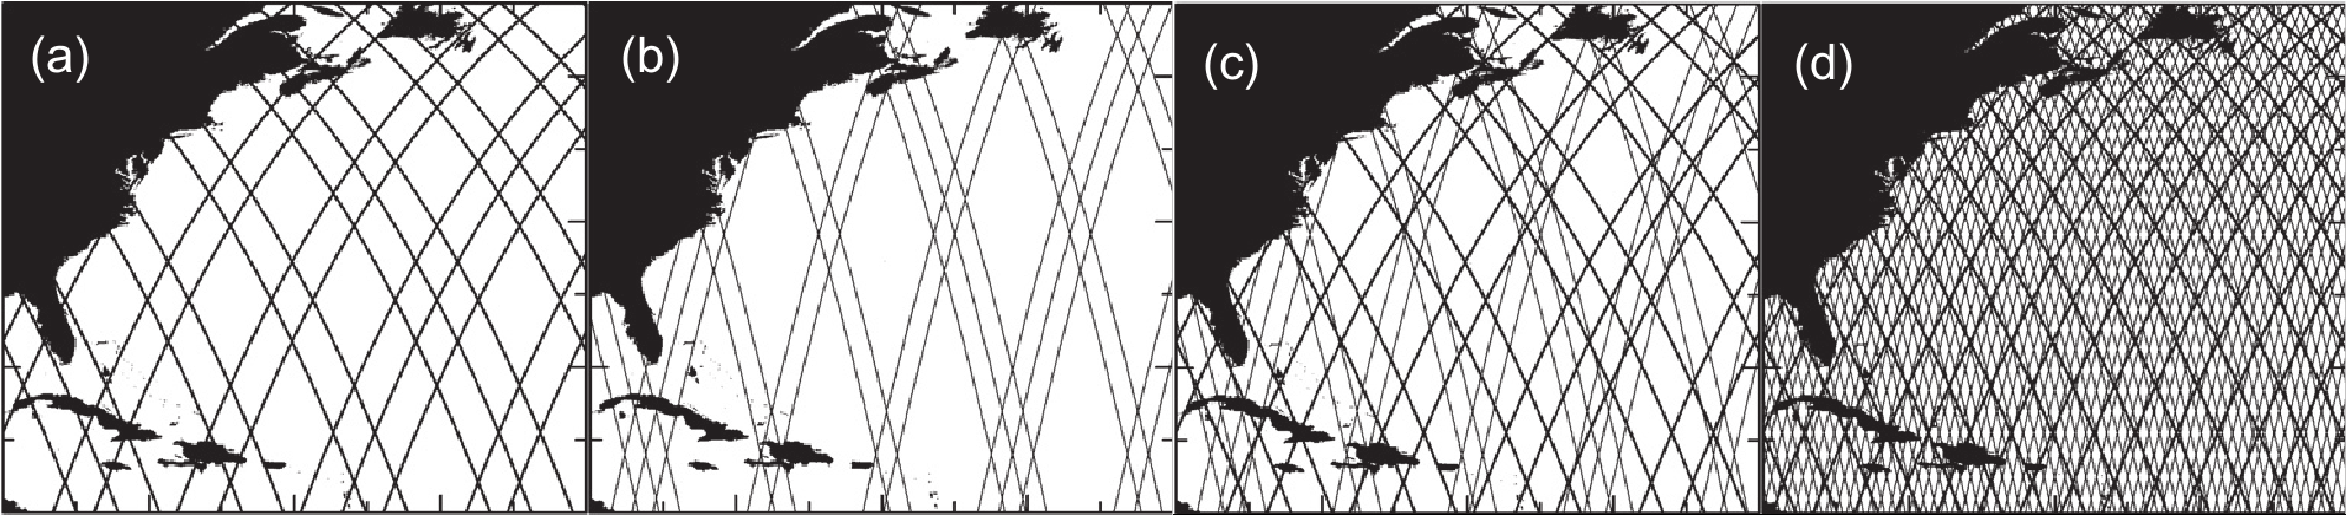
\includegraphics[]{tracks.pdf}
\caption[][-2cm]{The ground track patterns for the 10-day repeat orbit of T/P and its successors Jason-1 and Jason-2 (thick lines) and the 35-day repeat orbit of ERS-1 and its successors ERS-2 and Envisat (thin lines). (a) The ground tracks of the 10-day orbit during a representative 7-day period; (b) The ground tracks of the 35-day orbit during the same representative 7-day period; (c) The combined ground tracks of the 10-day orbit and the 35-day orbit during the 7-day period; and (d) The combined ground tracks of the 10-day orbit and the 35-day orbit during the full 35 days of the 35-day orbit. (sic) \citep{Chelton2011}}
\end{figure}

%\section[\Citeauthor{Chelton2007}~\citeyear{Chelton2007,Chelton2011}]{\SSH~Altimeter Data \citep{Chelton2007,Chelton2011}}\label{sec:hist_chelton}
\section*{\SSH~Altimeter Data \citep{Chelton2007,Chelton2011}}\label{sec:hist_chelton}
From the beginning of satellite altimetry \citeauthor{Chelton2011} have invested tremendous effort to thoroughly analyze the data in terms of
Rossby waves and geostrophic turbulence. At the time of the \citet{Killworth1997a} paper only 3 years of Topex/Poseidon data alone had been available,
which led them to interpret the data mainly in terms of Rossby waves. Once the merged Aviso T/P and ERS 1/2 \citep{Forget2010} was released 7 years later,
\citeauthor{Chelton2007} presented a new analysis that was based on an automated eddy-tracking algorithm using the geostrophic Okubo-Weiss parameter
\footnote{see \cref{subsec:detectmethods}.}\derref{der:okubo}. For the first time satellite data was resolved sufficiently fine to unveil the dominance of \textit{blobby
 structures rather than latitudinally $\dfdy$-refracted continuous crests and troughs} that had hitherto been assumed to characterize the large-scale \SSH~topography. They presented results of a refined algorithm in their \citeyear{Chelton2011} paper, in
which they abandoned the Okubo-Weiss concept and instead identified eddies via closed contours of \SSH~itself.
The improved algorithm and longer data record now allowed them to separate the non-linear eddy activity from the larger-scale Rossby waves. They find that the vast majority of extra-tropical westward propagating \SSH~variability does indeed consist of coherent, isolated, non-linear, mesoscale eddies that propagate about 25\% slower\footnote{pointing to dispersion.} than the linear waves.
Apart from this though they find little evidence for any dispersion in the signal,
neither do they find evidence for significant meridional propagation, as should be found for Rossby waves \citep[chapter 8.2.1]{olbers2012ocean}. In agreement with \citet{rhines1979theoretical}, they
find this eddy-dominated regime to fade towards the equator,
giving way to the characteristic Rossby wave profile. Almost all of their eddies propagate westwards. Those eddies that are advected eastwards by \eg the ACC show significantly shorter life-times than those that are not. For more detail on their results and a discussion of the limitations of eddy-tracking via satellites (see \cref{sec:satvsmod}).
